
%% bare_conf.tex
%% V1.3
%% 2007/01/11
%% by Michael Shell
%% See:
%% http://www.michaelshell.org/
%% for current contact information.
%%
%% This is a skeleton file demonstrating the use of IEEEtran.cls
%% (requires IEEEtran.cls version 1.7 or later) with an IEEE conference paper.
%%
%% Support sites:
%% http://www.michaelshell.org/tex/ieeetran/
%% http://www.ctan.org/tex-archive/macros/latex/contrib/IEEEtran/
%% and
%% http://www.ieee.org/

%%*************************************************************************
%% Legal Notice:
%% This code is offered as-is without any warranty either expressed or
%% implied; without even the implied warranty of MERCHANTABILITY or
%% FITNESS FOR A PARTICULAR PURPOSE! 
%% User assumes all risk.
%% In no event shall IEEE or any contributor to this code be liable for
%% any damages or losses, including, but not limited to, incidental,
%% consequential, or any other damages, resulting from the use or misuse
%% of any information contained here.
%%
%% All comments are the opinions of their respective authors and are not
%% necessarily endorsed by the IEEE.
%%
%% This work is distributed under the LaTeX Project Public License (LPPL)
%% ( http://www.latex-project.org/ ) version 1.3, and may be freely used,
%% distributed and modified. A copy of the LPPL, version 1.3, is included
%% in the base LaTeX documentation of all distributions of LaTeX released
%% 2003/12/01 or later.
%% Retain all contribution notices and credits.
%% ** Modified files should be clearly indicated as such, including **
%% ** renaming them and changing author support contact information. **
%%
%% File list of work: IEEEtran.cls, IEEEtran_HOWTO.pdf, bare_adv.tex,
%%          bare_conf.tex, bare_jrnl.tex, bare_jrnl_compsoc.tex
%%*************************************************************************

% *** Authors should verify (and, if needed, correct) their LaTeX system ***
% *** with the testflow diagnostic prior to trusting their LaTeX platform ***
% *** with production work. IEEE's font choices can trigger bugs that do ***
% *** not appear when using other class files.              ***
% The testflow support page is at:
% http://www.michaelshell.org/tex/testflow/



% Note that the a4paper option is mainly intended so that authors in
% countries using A4 can easily print to A4 and see how their papers will
% look in print - the typesetting of the document will not typically be
% affected with changes in paper size (but the bottom and side margins will).
% Use the testflow package mentioned above to verify correct handling of
% both paper sizes by the user's LaTeX system.
%
% Also note that the "draftcls" or "draftclsnofoot", not "draft", option
% should be used if it is desired that the figures are to be displayed in
% draft mode.
%
\documentclass[conference]{IEEEtran}
% Add the compsoc option for Computer Society conferences.
%
% If IEEEtran.cls has not been installed into the LaTeX system files,
% manually specify the path to it like:
% \documentclass[conference]{../sty/IEEEtran}





% Some very useful LaTeX packages include:
% (uncomment the ones you want to load)


% *** MISC UTILITY PACKAGES ***
%
%\usepackage{ifpdf}
% Heiko Oberdiek's ifpdf.sty is very useful if you need conditional
% compilation based on whether the output is pdf or dvi.
% usage:
% \ifpdf
%  % pdf code
% \else
%  % dvi code
% \fi
% The latest version of ifpdf.sty can be obtained from:
% http://www.ctan.org/tex-archive/macros/latex/contrib/oberdiek/
% Also, note that IEEEtran.cls V1.7 and later provides a builtin
% \ifCLASSINFOpdf conditional that works the same way.
% When switching from latex to pdflatex and vice-versa, the compiler may
% have to be run twice to clear warning/error messages.






% *** CITATION PACKAGES ***
%
%\usepackage{cite}
% cite.sty was written by Donald Arseneau
% V1.6 and later of IEEEtran pre-defines the format of the cite.sty package
% \cite{} output to follow that of IEEE. Loading the cite package will
% result in citation numbers being automatically sorted and properly
% "compressed/ranged". e.g., [1], [9], [2], [7], [5], [6] without using
% cite.sty will become [1], [2], [5]--[7], [9] using cite.sty. cite.sty's
% \cite will automatically add leading space, if needed. Use cite.sty's
% noadjust option (cite.sty V3.8 and later) if you want to turn this off.
% cite.sty is already installed on most LaTeX systems. Be sure and use
% version 4.0 (2003-05-27) and later if using hyperref.sty. cite.sty does
% not currently provide for hyperlinked citations.
% The latest version can be obtained at:
% http://www.ctan.org/tex-archive/macros/latex/contrib/cite/
% The documentation is contained in the cite.sty file itself.





\usepackage{graphicx}
\usepackage{float}
\usepackage{afterpage}
\usepackage{hyperref}
\usepackage{listings}

% *** GRAPHICS RELATED PACKAGES ***
%
%\ifCLASSINFOpdf
%\usepackage[pdftex]{graphicx}
 % declare the path(s) where your graphic files are
 % \graphicspath{{../pdf/}{../jpeg/}}
 % and their extensions so you won't have to specify these with
 % every instance of \includegraphics
 % \DeclareGraphicsExtensions{.pdf,.jpeg,.png}
%\else
 % or other class option (dvipsone, dvipdf, if not using dvips). graphicx
 % will default to the driver specified in the system graphics.cfg if no
 % driver is specified.
 % \usepackage[dvips]{graphicx}
 % declare the path(s) where your graphic files are
 % \graphicspath{{../eps/}}
 % and their extensions so you won't have to specify these with
 % every instance of \includegraphics
 % \DeclareGraphicsExtensions{.eps}
%\fi
% graphicx was written by David Carlisle and Sebastian Rahtz. It is
% required if you want graphics, photos, etc. graphicx.sty is already
% installed on most LaTeX systems. The latest version and documentation can
% be obtained at: 
% http://www.ctan.org/tex-archive/macros/latex/required/graphics/
% Another good source of documentation is "Using Imported Graphics in
% LaTeX2e" by Keith Reckdahl which can be found as epslatex.ps or
% epslatex.pdf at: http://www.ctan.org/tex-archive/info/
%
% latex, and pdflatex in dvi mode, support graphics in encapsulated
% postscript (.eps) format. pdflatex in pdf mode supports graphics
% in .pdf, .jpeg, .png and .mps (metapost) formats. Users should ensure
% that all non-photo figures use a vector format (.eps, .pdf, .mps) and
% not a bitmapped formats (.jpeg, .png). IEEE frowns on bitmapped formats
% which can result in "jaggedy"/blurry rendering of lines and letters as
% well as large increases in file sizes.
%
% You can find documentation about the pdfTeX application at:
% http://www.tug.org/applications/pdftex





% *** MATH PACKAGES ***
%
%\usepackage[cmex10]{amsmath}
% A popular package from the American Mathematical Society that provides
% many useful and powerful commands for dealing with mathematics. If using
% it, be sure to load this package with the cmex10 option to ensure that
% only type 1 fonts will utilized at all point sizes. Without this option,
% it is possible that some math symbols, particularly those within
% footnotes, will be rendered in bitmap form which will result in a
% document that can not be IEEE Xplore compliant!
%
% Also, note that the amsmath package sets \interdisplaylinepenalty to 10000
% thus preventing page breaks from occurring within multiline equations. Use:
%\interdisplaylinepenalty=2500
% after loading amsmath to restore such page breaks as IEEEtran.cls normally
% does. amsmath.sty is already installed on most LaTeX systems. The latest
% version and documentation can be obtained at:
% http://www.ctan.org/tex-archive/macros/latex/required/amslatex/math/





% *** SPECIALIZED LIST PACKAGES ***
%
%\usepackage{algorithmic}
% algorithmic.sty was written by Peter Williams and Rogerio Brito.
% This package provides an algorithmic environment fo describing algorithms.
% You can use the algorithmic environment in-text or within a figure
% environment to provide for a floating algorithm. Do NOT use the algorithm
% floating environment provided by algorithm.sty (by the same authors) or
% algorithm2e.sty (by Christophe Fiorio) as IEEE does not use dedicated
% algorithm float types and packages that provide these will not provide
% correct IEEE style captions. The latest version and documentation of
% algorithmic.sty can be obtained at:
% http://www.ctan.org/tex-archive/macros/latex/contrib/algorithms/
% There is also a support site at:
% http://algorithms.berlios.de/index.html
% Also of interest may be the (relatively newer and more customizable)
% algorithmicx.sty package by Szasz Janos:
% http://www.ctan.org/tex-archive/macros/latex/contrib/algorithmicx/




% *** ALIGNMENT PACKAGES ***
%
%\usepackage{array}
% Frank Mittelbach's and David Carlisle's array.sty patches and improves
% the standard LaTeX2e array and tabular environments to provide better
% appearance and additional user controls. As the default LaTeX2e table
% generation code is lacking to the point of almost being broken with
% respect to the quality of the end results, all users are strongly
% advised to use an enhanced (at the very least that provided by array.sty)
% set of table tools. array.sty is already installed on most systems. The
% latest version and documentation can be obtained at:
% http://www.ctan.org/tex-archive/macros/latex/required/tools/


%\usepackage{mdwmath}
%\usepackage{mdwtab}
% Also highly recommended is Mark Wooding's extremely powerful MDW tools,
% especially mdwmath.sty and mdwtab.sty which are used to format equations
% and tables, respectively. The MDWtools set is already installed on most
% LaTeX systems. The lastest version and documentation is available at:
% http://www.ctan.org/tex-archive/macros/latex/contrib/mdwtools/


% IEEEtran contains the IEEEeqnarray family of commands that can be used to
% generate multiline equations as well as matrices, tables, etc., of high
% quality.


%\usepackage{eqparbox}
% Also of notable interest is Scott Pakin's eqparbox package for creating
% (automatically sized) equal width boxes - aka "natural width parboxes".
% Available at:
% http://www.ctan.org/tex-archive/macros/latex/contrib/eqparbox/





% *** SUBFIGURE PACKAGES ***
%\usepackage[tight,footnotesize]{subfigure}
% subfigure.sty was written by Steven Douglas Cochran. This package makes it
% easy to put subfigures in your figures. e.g., "Figure 1a and 1b". For IEEE
% work, it is a good idea to load it with the tight package option to reduce
% the amount of white space around the subfigures. subfigure.sty is already
% installed on most LaTeX systems. The latest version and documentation can
% be obtained at:
% http://www.ctan.org/tex-archive/obsolete/macros/latex/contrib/subfigure/
% subfigure.sty has been superceeded by subfig.sty.



%\usepackage[caption=false]{caption}
%\usepackage[font=footnotesize]{subfig}
% subfig.sty, also written by Steven Douglas Cochran, is the modern
% replacement for subfigure.sty. However, subfig.sty requires and
% automatically loads Axel Sommerfeldt's caption.sty which will override
% IEEEtran.cls handling of captions and this will result in nonIEEE style
% figure/table captions. To prevent this problem, be sure and preload
% caption.sty with its "caption=false" package option. This is will preserve
% IEEEtran.cls handing of captions. Version 1.3 (2005/06/28) and later 
% (recommended due to many improvements over 1.2) of subfig.sty supports
% the caption=false option directly:
%\usepackage[caption=false,font=footnotesize]{subfig}
%
% The latest version and documentation can be obtained at:
% http://www.ctan.org/tex-archive/macros/latex/contrib/subfig/
% The latest version and documentation of caption.sty can be obtained at:
% http://www.ctan.org/tex-archive/macros/latex/contrib/caption/




% *** FLOAT PACKAGES ***
%
%\usepackage{fixltx2e}
% fixltx2e, the successor to the earlier fix2col.sty, was written by
% Frank Mittelbach and David Carlisle. This package corrects a few problems
% in the LaTeX2e kernel, the most notable of which is that in current
% LaTeX2e releases, the ordering of single and double column floats is not
% guaranteed to be preserved. Thus, an unpatched LaTeX2e can allow a
% single column figure to be placed prior to an earlier double column
% figure. The latest version and documentation can be found at:
% http://www.ctan.org/tex-archive/macros/latex/base/



%\usepackage{stfloats}
% stfloats.sty was written by Sigitas Tolusis. This package gives LaTeX2e
% the ability to do double column floats at the bottom of the page as well
% as the top. (e.g., "\begin{figure*}[!b]" is not normally possible in
% LaTeX2e). It also provides a command:
%\fnbelowfloat
% to enable the placement of footnotes below bottom floats (the standard
% LaTeX2e kernel puts them above bottom floats). This is an invasive package
% which rewrites many portions of the LaTeX2e float routines. It may not work
% with other packages that modify the LaTeX2e float routines. The latest
% version and documentation can be obtained at:
% http://www.ctan.org/tex-archive/macros/latex/contrib/sttools/
% Documentation is contained in the stfloats.sty comments as well as in the
% presfull.pdf file. Do not use the stfloats baselinefloat ability as IEEE
% does not allow \baselineskip to stretch. Authors submitting work to the
% IEEE should note that IEEE rarely uses double column equations and
% that authors should try to avoid such use. Do not be tempted to use the
% cuted.sty or midfloat.sty packages (also by Sigitas Tolusis) as IEEE does
% not format its papers in such ways.





% *** PDF, URL AND HYPERLINK PACKAGES ***
%
%\usepackage{url}
% url.sty was written by Donald Arseneau. It provides better support for
% handling and breaking URLs. url.sty is already installed on most LaTeX
% systems. The latest version can be obtained at:
% http://www.ctan.org/tex-archive/macros/latex/contrib/misc/
% Read the url.sty source comments for usage information. Basically,
% \url{my_url_here}.





% *** Do not adjust lengths that control margins, column widths, etc. ***
% *** Do not use packages that alter fonts (such as pslatex).     ***
% There should be no need to do such things with IEEEtran.cls V1.6 and later.
% (Unless specifically asked to do so by the journal or conference you plan
% to submit to, of course. )

%bib
\bibliographystyle{IEEEtran}

% correct bad hyphenation here
\hyphenation{op-tical net-works semi-conduc-tor}

% path to figures
\graphicspath{{figures/}}

\begin{document}
%
% paper title
% can use linebreaks \\ within to get better formatting as desired
\title{Web Application Model Generation \\through Crawling and UI Pattern Inferring}

% author names and affiliations
% use a multiple column layout for up to three different
% affiliations
\author{\IEEEauthorblockN{Clara Sacramento, Ana C. R. Paiva}
\IEEEauthorblockA{Departamento de Engenharia Informática\\
Faculdade de Engenharia da Universidade do Porto\\
Porto, Portugal\\
ei09090@fe.up.pt; apaiva@fe.up.pt; }}
%\and
%\IEEEauthorblockN{Homer Simpson}
%\IEEEauthorblockA{Twentieth Century Fox\\
%Springfield, USA\\
%Email: homer@thesimpsons.com}}
%\and
%\IEEEauthorblockN{James Kirk\\ and Montgomery Scott}
%\IEEEauthorblockA{Starfleet Academy\\
%San Francisco, California 96678-2391\\
%Telephone: (800) 555--1212\\
%Fax: (888) 555--1212}}

% conference papers do not typically use \thanks and this command
% is locked out in conference mode. If really needed, such as for
% the acknowledgment of grants, issue a \IEEEoverridecommandlockouts
% after \documentclass

% for over three affiliations, or if they all won't fit within the width
% of the page, use this alternative format:
% 
%\author{\IEEEauthorblockN{Michael Shell\IEEEauthorrefmark{1},
%Homer Simpson\IEEEauthorrefmark{2},
%James Kirk\IEEEauthorrefmark{3}, 
%Montgomery Scott\IEEEauthorrefmark{3} and
%Eldon Tyrell\IEEEauthorrefmark{4}}
%\IEEEauthorblockA{\IEEEauthorrefmark{1}School of Electrical and Computer Engineering\\
%Georgia Institute of Technology,
%Atlanta, Georgia 30332--0250\\ Email: see http://www.michaelshell.org/contact.html}
%\IEEEauthorblockA{\IEEEauthorrefmark{2}Twentieth Century Fox, Springfield, USA\\
%Email: homer@thesimpsons.com}
%\IEEEauthorblockA{\IEEEauthorrefmark{3}Starfleet Academy, San Francisco, California 96678-2391\\
%Telephone: (800) 555--1212, Fax: (888) 555--1212}
%\IEEEauthorblockA{\IEEEauthorrefmark{4}Tyrell Inc., 123 Replicant Street, Los Angeles, California 90210--4321}}




% use for special paper notices
%\IEEEspecialpapernotice{(Invited Paper)}




% make the title area
\maketitle


\begin{abstract}
%\boldmath
A great deal of effort in model-based testing is related to the creation of the model. The model itself, while a powerful tool of abstraction, can be a source of bugs. This paper presents a dynamic reverse engineering approach that aims to extract part of the model of an existing Web application through the identification of User Interface (UI) patterns. This approach explores the Web application via crawling, saves information related to the interaction (crawl history, HTML pages and their URLs), analyzes the gathered information, and infers the UI patterns via a set of heuristics rules.
\end{abstract}
\begin{IEEEkeywords} Reverse Engineering, Web Application, UI Patterns, Web Scraping, Web Crawling \end{IEEEkeywords}
% IEEEtran.cls defaults to using nonbold math in the Abstract.
% This preserves the distinction between vectors and scalars. However,
% if the conference you are submitting to favors bold math in the abstract,
% then you can use LaTeX's standard command \boldmath at the very start
% of the abstract to achieve this. Many IEEE journals/conferences frown on
% math in the abstract anyway.

% no keywords




% For peer review papers, you can put extra information on the cover
% page as needed:
% \ifCLASSOPTIONpeerreview
% \begin{center} \bfseries EDICS Category: 3-BBND \end{center}
% \fi
%
% For peerreview papers, this IEEEtran command inserts a page break and
% creates the second title. It will be ignored for other modes.
\IEEEpeerreviewmaketitle



\section{Introduction}
% no \IEEEPARstart
%This demo file is intended to serve as a ``starter file''
%for IEEE conference papers produced under \LaTeX\ using
%IEEEtran.cls version 1.7 and later.
% You must have at least 2 lines in the paragraph with the drop letter
% (should never be an issue)
%I wish you the best of success.

%\hfill horizontal fill
 
%\hfill January 11, 2007

Web applications are getting more and more important, and can now handle tasks that before could only be performed by desktop applications \cite{garrett2005ajax}, like editing images or creating spreadsheet documents. However, despite their growing relevance, they still suffer from a lack of standards and conventions \cite{constantine2002usage}, unlike desktop and mobile applications. This means that the same task can be implemented in many different ways, which makes automated testing difficult to accomplish and inhibits reuse of testing code.

GUIs (Graphical User Interfaces) of all kinds are populated with recurring behaviors that vary slightly. For example, authentication (\textit{login/password}) is a common behavior in many software applications. These behaviors (patterns) are called User Interface (UI) patterns \cite{van2001patterns} and are recurring solutions that solve common design problems. Due to their widespread use, UI patterns allow users a sense of familiarity and comfort when using applications. 

However, while UI patterns are familiar to users, their implementation may vary significantly. For a login, in some cases an error message may appear when the authentication fails; in others, the software application simply erases the inserted data and doesn’t send a message to the user. Despite this, it is possible to define generic and reusable test strategies to test them after a configuration process to adapt the tests to those different possible applications \cite{morgado2012gui}. 

That is the main idea behind the PBGT (\textit{Pattern-based GUI Testing}) project, in which this research work is developed. In the PBGT approach, the user builds a test model containing instantiations of UI patterns, and later uses that model to test their occurrences on Web applications.  The goal of the work described in this paper is to continue the work done in \cite{nabuco2013inferring} on the extraction process (PARADIGM-RE), where a reverse engineering process was developed to automatically identify the presence of UI Patterns on existent Web applications, provided the user interacts manually with the Web application with Selenium IDE \footnote{Selenium IDE: \url{http://docs.seleniumhq.org/docs/02_selenium_ide.jsp}} recording his actions. The work described in this paper aims to automatize the process: crawl a Web application, search for UI patterns in its pages, and finally produce a model with the results of the search.

The rest of the paper is structured as follows. Section \ref{sec:pbgt} presents an overview of the PBGT project, setting the context for this work. Section \ref{sec:sota} addresses the related work, as well as the tools available to perform the needed tasks. Section \ref{sec:imp} describes how the system was implemented. Section \ref{sec:eval} provides a practical example of the system proposed. Section \ref{sec:conclusion} provides the conclusions, reports some of the problems found and points out the future work. 

\section{PBGT Overview}\label{sec:pbgt}

\subsection{Architecture}

As mentioned before, the focus of this article is a component of an investigation project named PBGT (\textit{Pattern-based GUI Testing}) \cite{moreira2013pattern}. The goal of this investigation project is to develop a model-based GUI testing tool and approach, usable as an industrial tool. This project has five parts: a DSL (\textit{Domain Specific Language}) named \textbf{PARADIGM} to define GUI testing models based on UI patterns; \textbf{PARADIGM-RE}, a Web application reverse engineering tool whose purpose is to extract UI patterns from Web pages without access to their source code, and use the extracted patterns to generate a test model defined in PARADIGM; a modeling and testing environment, named \textbf{PARADIGM-ME}, made to support the creation of test models; an automatic test case generation tool, named \textbf{PARADIGM-TG}, that generates test cases from test models defined in PARADIGM; and finally a test case execution tool, named \textbf{PARADIGM-TE}, which executes test cases, analyzes their coverage, and returns detailed execution reports. The architecture and workflow of the project can better be seen in Fig. \ref{fig:pbgt}. Activities with cogs are automatic, and activities with stickmen require user input.

\begin{figure}[!ht]
\centering
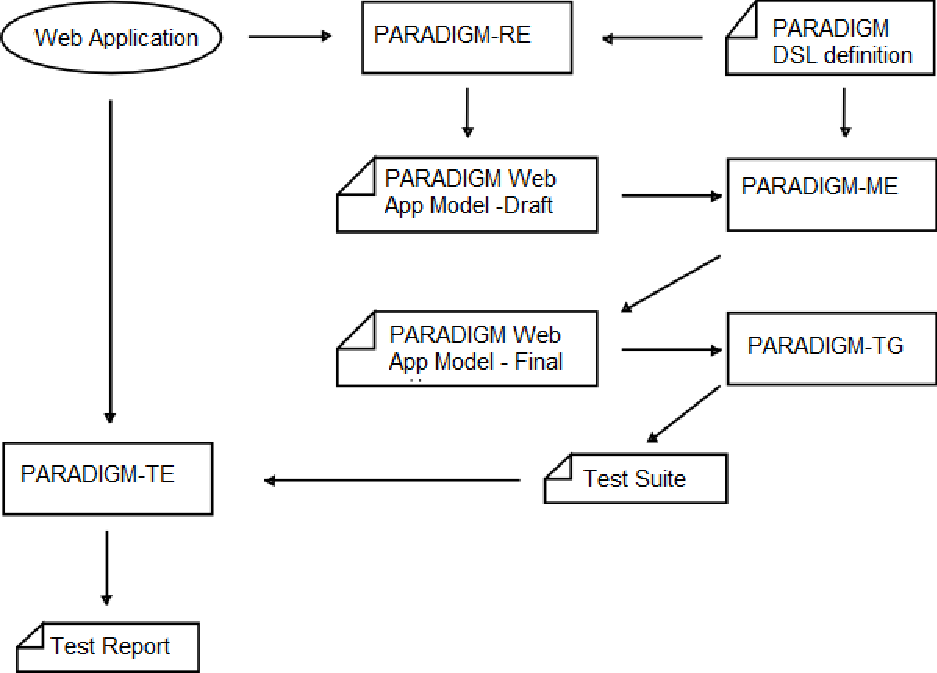
\includegraphics[width=0.5\textwidth]{pbgt}
\caption[An overview of the PBGT project]{An overview of the PBGT project \cite{nabuco2013inferring}}
\label{fig:pbgt}
\end{figure}

%\afterpage{
\subsection{Supported Patterns}
The UI Patterns defined in the PARADIGM language, and therefore supported by PARADIGM-RE, are:
\begin{description}
\item[\textit{Login}] \hfill \\
This pattern is commonly found in Web applications, especially in the ones that restrict access to functionalities or data. Usually consists of two input fields (a normal input box for email or username, and a cyphered text for the password) and a submit button, with optionally a ``remember me'' checkbox, to save the authentication data for the next visits. The authentication process has two possible outcomes: valid and invalid. Some websites may also include captcha verification upon too many failed login attempts.
\item[\textit{Search}] \hfill \\
This pattern consists of one or more input fields, where the user inserts keywords to search, and a submit button to start the search. The search may be submitted dynamically, and the submit button be omitted. Upon success, the website shows a list of results; upon failure, an error message may be shown.
\item[\textit{Sort}] \hfill \\
This pattern sorts a list of data by a common attribute (price, name and relevance) according to a defined criteria (ascending or descending, alphabetically, etc.). For example, in a Web store a user can sort a list of a specific type of products according to their price in order to identify the cheapest one.
\item[\textit{Master Detail}] \hfill \\
This pattern is present in a webpage when selecting an element from a set results in filtering/updating another related set accordingly. For example, clicking on a checkbox associated to a brand may include (or exclude) products of that brand in a product search result list. The set of selectable elements is called \textit{master} and the updated list is called \textit{detail}. Generally the only elements updated are the elements belonging to the \textit{detail} set.
\item[\textit{Menu}] \hfill \\
This pattern is very common in webpages. It's usually defined as a tree structure with several navigational options, to provide easier access for users. 
\item[\textit{Input}] \hfill \\
This pattern is any kind of input field that allows the user to insert data. May be a text box or textarea element.
\item[\textit{Call}] \hfill \\
This pattern is any kind of element where a click triggers a change of page. May be a link or a button.
\end{description}
%}

\subsection{Produced Models}

The models produced by PARADIGM-RE after the RE process consist of a XML file that contains all the information about the UI Patterns found: their definition and configurations. The PARADIGM model generated by the RE tool does not contain the connectors between the UI Patterns, only the UI Patterns and their configurations. These models are meant to be loaded to the PARADIGM-ME tool and completed manually.\\

%\fontsize{8pt}{9pt}\selectfont
%\lstset{language=XML,caption={An example of a .paradigm file with identified patterns},label=lst:paradigm,captionpos=b}
%\begin{lstlisting}[frame=single]
%<?xml version="1.0" encoding="UTF-8"?>
%<Paradigm:Model xmi:version="2.0" 
 % xmlns:xmi="http://www.omg.org/XMI"
  %xmlns:Paradigm="http://www.example.org/Paradigm" 
  %title="patterns"/>
	%<nodes xsi:type="Paradigm:Init" 
	    %name="XInit" number="1"/>
	%<nodes xsi:type="Paradigm:Search" 
	    %name="Search1" number="2"/>
	%<nodes xsi:type="Paradigm:Sort" 
	    %name="Sort1" number="3"/>
	%<nodes xsi:type="Paradigm:End" 
	    %name="End" number="4"/>
%</Paradigm:Model>
%\end{lstlisting}

%\fontsize{10pt}{9pt}\selectfont

\section{Crawling Approach}\label{sec:imp}


\section{Evaluation}\label{sec:eval}

%\subsection{Subsection Heading Here}
%Subsection text here.


%\subsubsection{Subsubsection Heading Here}
%Subsubsection text here.


% An example of a floating figure using the graphicx package.
% Note that \label must occur AFTER (or within) \caption.
% For figures, \caption should occur after the \includegraphics.
% Note that IEEEtran v1.7 and later has special internal code that
% is designed to preserve the operation of \label within \caption
% even when the captionsoff option is in effect. However, because
% of issues like this, it may be the safest practice to put all your
% \label just after \caption rather than within \caption{}.
%
% Reminder: the "draftcls" or "draftclsnofoot", not "draft", class
% option should be used if it is desired that the figures are to be
% displayed while in draft mode.
%
%\begin{figure}[!t]
%\centering
%\includegraphics[width=2.5in]{myfigure}
% where an .eps filename suffix will be assumed under latex, 
% and a .pdf suffix will be assumed for pdflatex; or what has been declared
% via \DeclareGraphicsExtensions.
%\caption{Simulation Results}
%\label{fig_sim}
%\end{figure}

% Note that IEEE typically puts floats only at the top, even when this
% results in a large percentage of a column being occupied by floats.


% An example of a double column floating figure using two subfigures.
% (The subfig.sty package must be loaded for this to work.)
% The subfigure \label commands are set within each subfloat command, the
% \label for the overall figure must come after \caption.
% \hfil must be used as a separator to get equal spacing.
% The subfigure.sty package works much the same way, except \subfigure is
% used instead of \subfloat.
%
%\begin{figure*}[!t]
%\centerline{\subfloat[Case I]\includegraphics[width=2.5in]{subfigcase1}%
%\label{fig_first_case}}
%\hfil
%\subfloat[Case II]{\includegraphics[width=2.5in]{subfigcase2}%
%\label{fig_second_case}}}
%\caption{Simulation results}
%\label{fig_sim}
%\end{figure*}
%
% Note that often IEEE papers with subfigures do not employ subfigure
% captions (using the optional argument to \subfloat), but instead will
% reference/describe all of them (a), (b), etc., within the main caption.


% An example of a floating table. Note that, for IEEE style tables, the 
% \caption command should come BEFORE the table. Table text will default to
% \footnotesize as IEEE normally uses this smaller font for tables.
% The \label must come after \caption as always.
%
%\begin{table}[!t]
%% increase table row spacing, adjust to taste
%\renewcommand{\arraystretch}{1.3}
% if using array.sty, it might be a good idea to tweak the value of
% \extrarowheight as needed to properly center the text within the cells
%\caption{An Example of a Table}
%\label{table_example}
%\centering
%% Some packages, such as MDW tools, offer better commands for making tables
%% than the plain LaTeX2e tabular which is used here.
%\begin{tabular}{|c||c|}
%\hline
%One & Two\\
%\hline
%Three & Four\\
%\hline
%\end{tabular}
%\end{table}


% Note that IEEE does not put floats in the very first column - or typically
% anywhere on the first page for that matter. Also, in-text middle ("here")
% positioning is not used. Most IEEE journals/conferences use top floats
% exclusively. Note that, LaTeX2e, unlike IEEE journals/conferences, places
% footnotes above bottom floats. This can be corrected via the \fnbelowfloat
% command of the stfloats package.

\section{Related Work}\label{sec:sota}

Reverse engineering is ``the process of analyzing the subject system to identify the system components and interrelationships and to create representations of the system in another form or at a higher level of abstraction'' \cite{chikofsky1990reverse}. There are two methods of applying reverse engineering to a system: the dynamic method, in which the data are retrieved from the system at run time without access to the source code, and the static method, which obtains the data from the system source code \cite{systa1999dynamic}. There is also the hybrid method, which combines the two previous methods, and the historical method, which includes historic information to see the evolution of the software system \cite{canfora2011achievements}. These approaches follow the same main steps: collect the data, analyze it and represent it in a legible way, and in the process allow the discovery of information about the system's control and data flow \cite{pacione2003comparative}.

There are plenty of approaches that extract information from Web applications \cite{elbaum2003improving,sampath2007applying,amalfitano2010rich, andjelkovic2011trace}. ReGUI \cite{coimbra2011reverse,coimbra2012dynamic} is a dynamic reverse engineering tool made to reduce the effort of modeling the structure and behavior of a software application GUI. Duarte, Kramer and Uchitel defined an approach for behavior model extraction which combines static and dynamic information \cite{duarte2006model}.

In the area of Web crawling, there are many open source crawlers, the most notable being Apache Nutch \footnote{Apache Nutch: \url{http://nutch.apache.org/}}, Bixo \footnote{Bixo: \url{http://bixo.101tec.com/}}, Heritrix \footnote{Heritrix: \url{http://bit.ly/1dYRV2n}}, Crawler4j \footnote{Crawler4j: \url{http://code.google.com/p/crawler4j/}}, and Scrapy \footnote{Scrapy: \url{http://scrapy.org}}. We must also consider HTML parsers and extractors, to process the crawling results. Scrapy, being a crawling and scraping framework, counts on both lists. Other notable parsers are Mechanize \footnote{Mechanize (Python version): \url{http://wwwsearch.sourceforge.net/mechanize/}}, and Beautiful Soup \footnote{Beautiful Soup: \url{http://bit.ly/1iVZlbl)}}.

There are also plenty of approaches that crawl a Web application, and in the process extract information. Crawljax \cite{roest2010automated} is a tool that obtains graphical site maps by automatically crawling through a Web application. Mesbah \textit{et al.} proposed an automated technique for generating test cases with invariants from models inferred through dynamic crawling \cite{mesbah2012invariant}. Another approach by Mesbah \textit{et al.}, named FeedEx \cite{fard2013feedback} is a feedback-directed Web application exploration technique to derive test models. It uses a greedy algorithm to partially crawl a RIA's GUI, and the goal is that the derived test model capture different aspects of the given Web application's client-side functionality. WebDiff \cite{choudhary2010Webdiff} is a tool that searches for cross-browser inconsistencies by analyzing a website's DOM and comparing screenshots obtained in different browsers. Dincturk \textit{et al.} \cite{dincturk2012statistical} proposed a RIA crawling strategy using a statistical model based on the model-based crawling approach introduced in \cite{benjamin2011strategy} to crawl RIAs efficiently. Dallmeier \textit{et al.}'s Webmate \cite{dallmeier2012Webmate,dallmeier2013Webmate} is a tool that analyzes the Web application under test, identifies all functionally different states, and is then able to navigate to each of these states at the user’s request.

User Interaction (UI) patterns, in particular the ones supported by the tool, are well-documented in a various number of sources \cite{tidwell2010designing,van2001patterns, neil12standard,sinnig2005patterns}. Lin and Landay's approach \cite{lin2008employing} uses UI patterns for Web applications that run on PCs and mobile phones, and prompt-and-response style voice interfaces. Pontico \textit{et al.}'s approach \cite{pontico2008organizing} presents UI patterns common in eGovernment applications.

Despite the fact that there are plenty of approaches to mine patterns from Web applications, no approaches have been found that infer UI patterns from Web applications beside the work extended in this paper \cite{nabuco2013inferring, morgado2012gui}. The approaches found deal mostly with Web mining, with the goal of finding relationships between different data or finding the same data in different formats. Brin \cite{brin1999extracting} presented an approach to extract relations and patterns for the same data spread through many different formats. Chang \cite{chang2003automatic} proposes a similar method to discover patterns, by extracting structured data from semi-structured Web documents. Freitag \cite{freitag1998information} proposed a general-purpose relational learner for information extraction from Web applications.

%\section{Conclusion}\label{sec:conclusion}
%The conclusion goes here.




% conference papers do not normally have an appendix


% use section* for acknowledgement
%\section*{Acknowledgment}


%The authors would like to thank...





% trigger a \newpage just before the given reference
% number - used to balance the columns on the last page
% adjust value as needed - may need to be readjusted if
% the document is modified later
%\IEEEtriggeratref{8}
% The "triggered" command can be changed if desired:
%\IEEEtriggercmd{\enlargethispage{-5in}}

% references section

% can use a bibliography generated by BibTeX as a .bbl file
% BibTeX documentation can be easily obtained at:
% http://www.ctan.org/tex-archive/biblio/bibtex/contrib/doc/
% The IEEEtran BibTeX style support page is at:
% http://www.michaelshell.org/tex/ieeetran/bibtex/
%\bibliographystyle{IEEEtran}
% argument is your BibTeX string definitions and bibliography database(s)
%\bibliography{IEEEabrv,../bib/paper}
%
% <OR> manually copy in the resultant .bbl file
% set second argument of \begin to the number of references
% (used to reserve space for the reference number labels box)
%\begin{thebibliography}{1}

%\bibitem{IEEEhowto:kopka}
%H.~Kopka and P.~W. Daly, \emph{A Guide to \LaTeX}, 3rd~ed.\hskip 1em plus
 %0.5em minus 0.4em\relax Harlow, England: Addison-Wesley, 1999.

%\end{thebibliography}

\bibliography{bib}


% that's all folks
\end{document}


